\section{Einleitung} \label{sec:einleitung}

Im Rahmen dieser Aufgabenstellung wurden in zwei aufeinander aufbauenden Schritten ein Schaltnetzteil entworfen und die entsprechenden Maßnahmen zur elektromagnetischen Verträglichkeit (EMV) untersucht. Im ersten Teil bestand die Aufgabe darin, eine geregelte Schaltnetzteil-Schaltung in LTspice zu entwickeln, ohne ein Eingangsfilter zu implementieren. Im zweiten Schritt sollte die Schaltung hinsichtlich der leitungsgebundenen Emissionen (differenzielle und Gleichtaktstörungen) analysiert und ein geeignetes Filterdesign entwickelt werden, um die EMV-Tests zu bestehen.

Für die Umsetzung wurde der LTC3639 (Abbildung \ref{fig:LTC3639-1185}), ein Step-Down-Schaltregler von Analog Devices, verwendet. Die Simulationen wurden sowohl ohne als auch mit einem geeigneten Filter durchgeführt.


\begin{figure}[H]
    \centering
    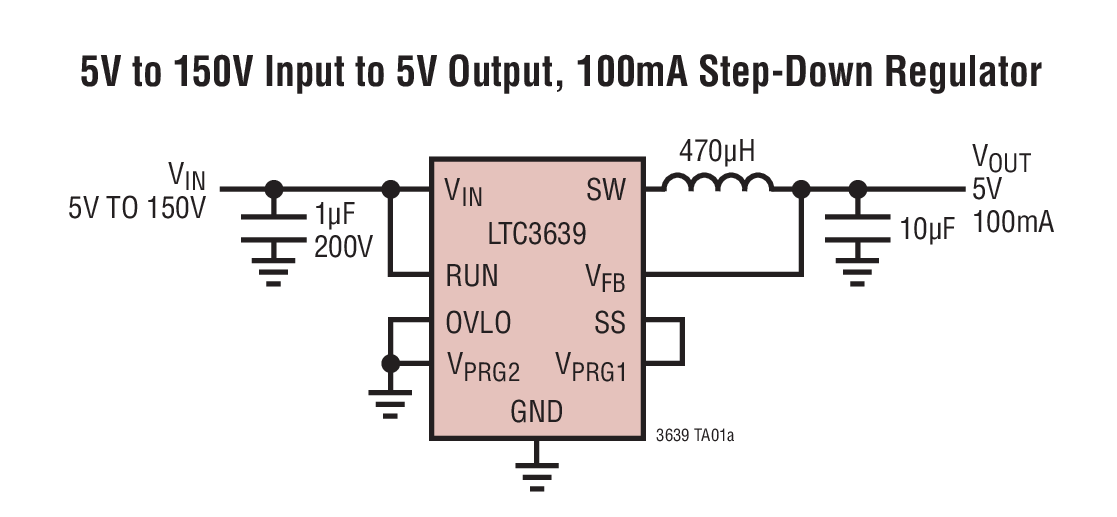
\includegraphics[width=0.8\linewidth]{document/Figure/LTC3639-1185.png}
    \caption{LTC3639-1185}
    \label{fig:LTC3639-1185}
\end{figure}